%\begin{savequote}[8cm]
%\textlatin{Jedem Anfang wohnt ein Zauber innne.}
%
%In the core of every beginning lives magic.
%  \qauthor{--- Hermann Hesse's \textit{Stufen}}
%\end{savequote}

\chapter{\label{ch:3-DCNs}Deep Counterfactual Networks} 

%\minitoc

\section{Motivation}
Deep neural networks represent one of the key areas of research in machine learning. They are responsible for a multitude of recent success in various fields such as computer vision and natural language processing. 

Despite their success, only limited research has been done on how to use deep neural networks for the task of counterfactual inference. However, recent results % CITE Sontag
have shown that neural networks can not only provide a valid option worth considering but is actually able to outperform the state-of-the-art. 

Nevertheless, there is a number of open questions when it comes to applying deep neural networks to counterfactual inference. Firstly, we have to deal with the problem of \emph{covariate shift}, i.e. the different distribution of the feature in the factual and counterfactual datasets respectively. Secondly, deep neural networks typically act as a black-box, lacking any kind of understandability or statistical interpretation. % LANG Does the words interpretablity exist? 
In particular, we are not able to provide confidence intervals with the respect to the quality of our prediction. While confidence intervals are a desired feature to have in almost every kind of task, they could be considered of crucial importance for the task of counterfactual inference: We just need to think of a doctor in a hospital who is using our model to generate actionable insights on whether or not to administer a certain treatment to a patient in need. Here, understandability is of key importance since the doctor needs to be able to trust the algorithm and potentially justify her decision that were based on the algorithm. 

In the following, we propose a model that we call \emph{deep counterfactual network} or (DCN) that conceptualises the counterfactual inference as a multi-task learning problem. In addition, we introduce novel dropout scheme that is based on the propensity score and allows a probabilistic interpretation of the model. 
\section{Model Description}
Previous models often followed the approach of \emph{direct modelling} in which a single-output regression model 
\begin{equation}
f: \mathcal{X} \times \{0,1\} \rightarrow \mathbb{R}
\end{equation}
is used to estimate the individualised treatment effect $T(x)$, with $\mathcal{X}$ being the population of contexts. In other words, the treatment assignment $W_i \in \{0,1\}$ for each subject is used as a bivariate input feature of the model. 

  The model is \emph{statistically efficient} in the sense that it makes use of the commonalities between the different response surfaces of the treated and untreated subjects. On the flip side, it sacrifices accuracy as it limits the interaction between the treatment assignment and the other features of the subject, in particular when dealing with  high-dimensional input data where the treatment assignment might simply get lost among the other features. Moreover, if the \emph{response surfaces} of the treated and untreated subjects differ significantly (e.g. features that are relevant to one outcome are are significant for the other outcome and vice versa), the model performs poorly and the consequences can be severe. 

A competing previous approach called \emph{virtual twin} uses two completely separate models to fit the treated and untreated population. % CITE Lu at al. 
While this approach has a high modelling flexibility and expressiveness for both outcomes, it sacrifices its \emph{statistical efficiency} as both outcome models are completely separated and therefore not able to reuse any of the correlations observed in the model for the respective other outcome. 




\begin{figure}[h]
	\centering
	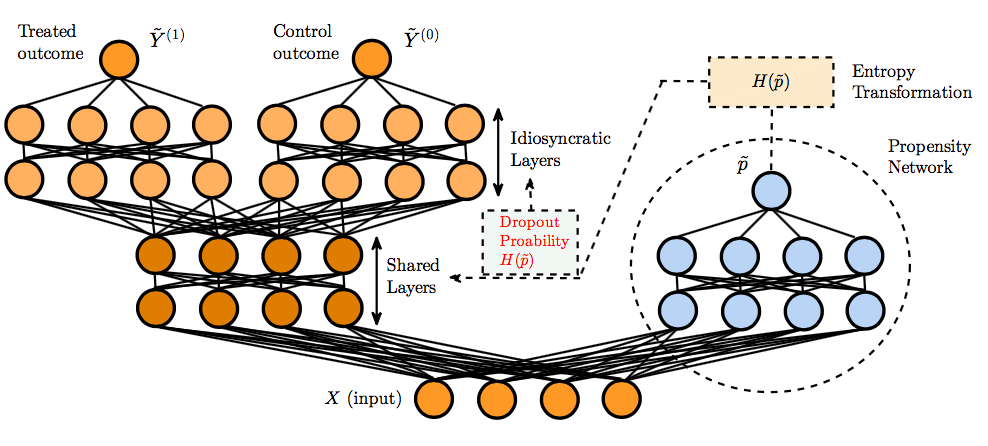
\includegraphics[width=1.0\textwidth]{figures/chapter-3/pbd-architecture.png}
	\caption{Architecture of Deep Counterfactual Networks}\label{fig:dcn-architecture}
\end{figure}

We introduce \emph{deep counterfactual networks} a novel approach to using deep neural networks for the task of counterfactual inference. Our model -- illustrated in figure \ref{fig:dcn-architecture} and described in detail in the following -- conceptualises counterfatual inference as a multi-task learning problem (see section \ref{sec:multi-task-learning}). This way, we achieve  statistical efficiency while at the same time ensuring a high degree of modelling flexibility. 

In addition, we address the  problem of the covariate shift between the factual and counterfactual dataset by utilising a novel propensity-based dropout scheme (see section \ref{sec:propensity-based-dropout}). This way, we are also able to provide confidence intervals for our predictions increasing. 

\subsection{Multi-Task Learning} \label{sec:multi-task-learning}
\emph{Deep counterfactual networks} (DPNs) make use of multi-task learning to learn a \emph{shared representation} for the potential outcomes (treated and untreated) in order to predict the individualised treatment effect $T(x)$. 

Our model, illustrated in figure \ref{fig:dcn-architecture}, consists of two separate networks: A \emph{propensity-network} on the right and a \emph{potential outcomes network} on the left.

The propensity-network represents a standard feed-forward neural network consisting of $L_p$ hidden layers and $h_p^{(l)}$ hidden units for the $l^{th}$ layer. It is trained separately and used to estimate the propensity scores for each sample $(X_i, W_i) \in \mathcal{D}$, thus treating the problem as a binary classification problem with the treatment assignment as target label. 

The \emph{outcome network} uses a multi-task architecture % CITE Collobert & Weston
with $L_s$ \emph{shared layers} (with $h_s^{(l)}$ hidden units in the $l^{th}$ layer) and $L_{i,j}$ \emph{outcome-specific layers} (with $h_{i,j}^{(l)}$ hidden units in the $l^{th}$ layer) for each outcome $j \in \{0,1\}$. This way, we treat the learning of the two outcome response surfaces $\mathbb{E}[Y_i^{(1)} \mid X_i = x]$ and $\mathbb{E}[Y_i^{(0)} \mid X_i = x]$ as two separate but related tasks that are learnt jointly in terms of a multi-task learning problem.

As a consequence, the training data $\mathcal{D}$ obtained from an observational study is separated into two task-specific subsets: a \emph{treated set} $\mathcal{D}^{(1)} = \{i \in \mathcal{D} : W_i = 1\}$ containing all treated subjects, and a \emph{control set} $\mathcal{D}^{(0)} = \{i \in \mathcal{D} : W_i = 0\}$ comprised of all untreated subjects. 

It is the purpose of the shared layers to capture any commonalities between the two outcome surfaces of both tasks. The shared layers also ensure a high level of statistical efficiency as they are able to make use of both datasets $\mathcal{D}^{(0)}$ and $\mathcal{D}^{(1)}$. 

In contrast, the outcome-specific layers allow the model to capture any individual complexity for each response surface. This is achieved by only using the subset $\mathcal{D}^{(j)}$ to learn the response surface $\mathbb{E}[Y_i^{(j)} \mid X_i = x]$, giving us a high level modelling flexibility that ensures accurate predictions even when the response surfaces differ significantly. 

Concluding, treating the problem of counterfactual inference as a multi-task learning problem enables us to train a flexible model that is able to capture potential individual for each response surface while at the same time ensuring an statistically efficient use the entire dataset for any shared complexity. 
	
\subsection{Propensity-based Dropout} \label{sec:propensity-based-dropout}
One of the key challenges of counterfactual inference is the problem of the \emph{covariate shift} (different distribution of the features) between the factual and counterfactual dataset which is caused by the selection bias of the treatment assignment policy.

In our model, we address this issue by applying a special regularisation technique that we will refer to as \emph{propensity-dropout} or PD. Propensity-dropout is based on regular dropout % CITE Hinton
that utilises the individual propensity score of a subject when training the model. In other words, for each individual sample we use a different dropout probability for the nodes in the network calculated as
\begin{equation}
P_{\text{dropout}}(x) = 1 - \frac{\lambda}{2} - \frac{1}{2} \mathbb{H}(\tilde{p}(x))
\end{equation}
where $\tilde{p}$ is the propensity score of subject $x$ as estimated by our \emph{propensity network}, $0 \leq \gamma \leq 1$ is an adjustable parameter (we typically use $\gamma = 1$), and $\mathbb{H}$ with
\begin{equation}
\mathbb{H} = -p \log (p) - (1-p)\log (1-p)
\end{equation}
refers to the entropy % CITE SHANNON
known from information theory. 

Consequently, a sample $x$ with an extreme propensity score ($\tilde{p}(x) = 0$ or $hat{p}(x) = 1$) receives a high dropout probability of $P_{\text{dropout}}(x) = 1 - \frac{\lambda}{2}$ (i.e. typically $0.5$), whereas samples with a balanced propensity score $hat{p}(x) = 0.5$ receive a low dropout probability $P_{\text{dropout}}(x) = \frac{1}{2} - \frac{\lambda}{2}$ (typically 0).

Intuitively, we want our dropout scheme to mask out hidden units in a way that assigns "simple models" to subjects with very high ($p(x)$ close to $1$) or low  ($p(x)$ close to $1$) propensity scores, whereas we want to assign more "complex models" to subjects that have a balanced propensity score ($p(x)$ close to $0.5$). In other words, the dropout probability will be higher for subjects with potentially unreliable features that belong to an area of small treatment assignment overlap in the feature space. This way, we penalise training sample with extreme propensity scores in order to prevent the network from co-adapting with potentially unreliable samples, allowing the model to generalise better to the actual distribution of features.

%Propensity-dropout represents a conceptual equivalent to propensity-weighting % CITE Abadie and Ibens
%that is applied on regular dropout. % CITE Srivstava et al 
 
Besides its regularising and balancing effect towards the covariate shift introduced by the selection bias, propensity dropout enables us to associate the estimated individualised treatment effects $\tilde{T}(x)$ with a corresponding measure of confidence. This can be achieved by utilising a Monte Carlo propensity-dropout scheme where we draw samples of $\tilde{T}(x)$  for our model. % CITE GAL & Ghahramani
In our model, a sample of $\tilde{T}(x)$  for a subject with features $x$ can be drawn as defined by:
\begin{flalign} % TODO DOUBLE CHECK THESE EQUATIONS!!!!!
	\tilde{p}(x) = f(...f((w_p^{(1)})^Tx)...) \\
	\mathbf{r}_s^{(l)}, \mathbf{r}_{i,0}^{(l)}, \mathbf{r}_{i,1}^{(l)} \sim Bernoulli(1-\frac{\lambda}{2} - \frac{1}{2}\mathbb{H}(\tilde{p}(x))) \\
	\tilde{s}(x) = f(...f(\mathbf{r}_s^{(1)}  \odot (\mathbf{w}_s^{(1)})^T x)...) \\
	\tilde{Y}^{(1)} = f(...f(\mathbf{r}_{i,1}^{(1)}  \odot (\mathbf{w}_{i,1}^{(1)})^T \tilde{s}(x))...) \\
	\tilde{Y}^{(0)} = f(...f(\mathbf{r}_{i,0}^{(1)}  \odot (\mathbf{w}_{i,0}^{(1)})^T \tilde{s}(x))...) \\			
	\tilde{T} = \tilde{Y}^{(1)} - \tilde{Y}^{(0)},
\end{flalign}
where $\mathbf{w}_p^{(l)}, \mathbf{w}_s^{(l)}, \mathbf{w}_{i,0}^{(l)},$ and $\mathbf{w}_{i,1}^{(l)}$ refer to the weight matrices for the $l^{th}$ respective propensity, shared, or outcome-specific layer; $\mathbf{r}_s^{(l)}, \mathbf{r}_{i,0}^{(l)},$ and $\mathbf{r}_{i,1}^{(l)}$ correspond to the dropout masks, and $f: \mathbb{R} \rightarrow \mathbb{R}$ is an arbitrary activation function (e.g. a ReLU or the logistic function). 

\section{Training the Model}
The network is trained in two alternating phases. In each phase, we use either the untreated samples $\mathcal{D}^{(0)}$ or the treated samples $\mathcal{D}^{(1)}$ as our training set to update the weights. 
% TODO Replace with actual algorithm!!!
\begin{figure}[h]
	\centering
	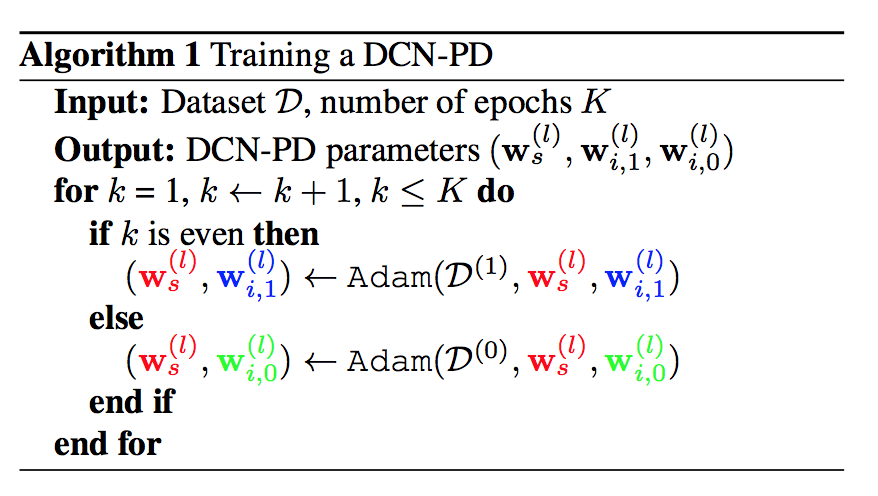
\includegraphics[width=0.6\textwidth]{figures/chapter-3/training-algorithm.png}
	\caption{Training Algorithm}\label{fig:training-algorithm}
\end{figure}
The algorithm is outlined in listing \ref{fig:training-algorithm} and can be described as follows: We train the model by iterating over a total $K$ epochs. In the even epochs ($k \mod 2 = 0$), we use $\mathcal{D}^{(1)}$ to update the weights of the outcome-specific layers of the treated subjects, in the odd epochs ($k \mod 2 \neq 0$) we update the outcome-specific layers of the control subjects. 

\begin{figure}[h]
	\centering
	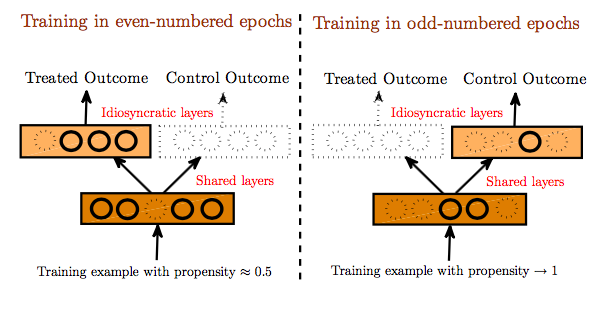
\includegraphics[width=0.8\textwidth]{figures/chapter-3/pbd-training.png}
	\caption{Visualisation of Training Algorithm}\label{fig:dcn-training}
\end{figure}


Note, how the weights of the shared layers are updated in every iteration. In order to update the weights, we are using the \emph{Adam optimiser} with \emph{Xavier initialisation}. % CITE Kingma & Ba
% TODO Consider if I should make it more general (why Adama?)

The deep counterfactual network is trained using the propensity-dropout (DP) described in the previous section and illustrated in figure \ref{fig:dcn-training} with $\lambda = 1$: The left-hand side depicts the training of a treated sample with a balanced propensity score, leading to only a few (if any) masked units, whereas the right-hand side illustrates the training of an untreated sample with a high propensity score which is highly regularised in order to ensure a balanced representation and effective generalisation of the model. The alternating training can be conceptualised as an application of a deterministic dropout masking out every unit of the outcome-specific layers of the currently untrained outcome.



